\documentclass{article}
\usepackage{amsmath}
\usepackage{graphicx}
\usepackage{float}
\usepackage{bm}
\usepackage{undertilde}
\usepackage{subfig}
\usepackage[a4paper, total={6in, 9in}]{geometry}
\renewcommand{\familydefault}{\sfdefault}

\title{Evolution of correlation between traits in a sexually recombining population within a single selective environment}
\date{June 2020}
\author{Simon Pirkl, Andreas Rohrbach}

\begin{document}

\maketitle

\begin{center}
	
\includegraphics[height=10mm]{./img/ci/HSWT_Logo_gruen.png}

	\vspace{5mm}
	Department of Bioengineering Sciences, Bioprocess Informatics
\end{center}

% \newpage

\tableofcontents
\newpage

\section{Abstract}

Watson et al. investigated the evolution of phenotypic correlations and "developmental memory". In one of their experiments, an evolutionary model was simulated, containing a single representative individual undergoing individual mutations. This simplification is legit under the assumption of SSWM (strong selection, weak mutation). 
To verify their results in a more realistic model of evolution involving sexual recombination, the experiment was replicated with a more sophisticated fitness evaluation and simple sexual recombination.

It was --Results--

--Discussion--

\section{Introduction}

The phenotypic variants we observe are not purely a product of their genes, but of multiple factors, with developmental processes being one of them \cite{laland2015}. In the work of Watson et al, the evolution of a network of recurrent nonlinear ontogenetic interactions was investigated \cite{watson2014}. Such a network could represent a gene regulation network. In their work, multiple experiments were conducted to better understand the evolution of such networks. In the first experiment, the basic effect of selection on interaction coefficients as a function of a single selective environment was assessed. This experiment was conducted under the assumptions of SSWM (strong selection, weak mutation), under which it is sufficient to model the evolution of just one representative individual undergoing individual mutations. 

One of Watson et al's results is that correlations in their single gene regulation network evolve according to Hebb’s rule \cite{hebb}, a simple associative neural learning mechanism, often summarized as "Cells that fire together wire together" \cite{shatz1992}.
Translated to genes and traits, it would state: if evolution selects a correlation of multiple gene states, those gene states will also become developmentally correlated (see also Pavlicev et al. 2011 \cite{pavlicev2011}).
This could be summarized as "traits that are selected together correlate together" \cite{watson2014}.

We aim to verify their findings in a population context with sexual recombination.
Since mutation and sexual recombination generate greater genetic variation, this could lead to correlations evolving not in accordance with Hebb's rule. However, we postulate that Hebb’s rule is driven not by mutation and recombination, but by selection.
If we reproduce Watson et al’s experiment 1 (single selective environment) for a network population with mutation and recombination, and our adaptive theory is correct, we predict that Hebb’s rule will apply to the evolved networks.

\section{Methods}

The population is modeled with individuals defined by their genotype, phenotype and gene regulation network. 
The evolution process is simulated by generating a new set of individuals through sexual recombination based on their previously developed adult phenotype, which is used to calculate the fitness. Furthermore the recombined individuals experiences a mutation before developing to their adult state.


\subsection{Gene regulation network}

As in the work of Watson et al, the gene regulation network (grn) is modeled as a two dimensional matrix $\bm{B}$, containing $nTrait * nTrait$ elements, with $nTrait$ being the number of genes and the number of corresponding traits as well.
Each element of the matrix contains the correlation coefficient between two genes/traits, and is in the range $[-1; +1]$, where 0 corresponds to no correlation at all, a negative coefficient indicating anticorrelation (or negative correlation), and a positive coefficient indicating positive correlation.

For the evaluation of the evolved gene reegulation networks, ...

To evalute our results, we used a matrix caluclated by Hebb's rule to recreate Watsons (2014) experiment 1. This is valid as Watson stated that incremental inheritable changes towards a given target agrees with the principles of neural learning mechanisms and therefore follows the Hebbian theory.

- selective environment

- r

\begin{equation}
	\Delta w_{ij} = r * s_i * s_j \\
	(r > 0)
\end{equation}

\subsection{Genotype and phenotype}

The genotype $\bm{G}$ and phenotype $\bm{P}$ are represented by column vectors with $nTrait$ elements. Each element contains a value in the range $[-1; 1]$ which represents the expression of the traits.

Each generation, for every individual, the genotype and gene regulation network is mutated by adding a value in a predefined range to one element.
The genotype is mutating faster within the range $[-0.1; 0.1]$ than the gene regulation network, which mutational increment is 1/15th of the genotype mutation range ($[-0.0067; 0.0067]$).

\subsection{Ontogenetic development}

In every generation the phenotypes have to be developed through time, influenced by the gene regulation network. The starting point is defined by the genotype. $\bm{P}(0) = \bm{G}$

After defining the initial phenotype, the development of individuals is represented by simulating through developmental time steps (set at $NDevSteps$ = 10). In each timestep the phenotype experiences the influence of the gene regulation network, calculated by the formula: 

\begin{equation}
	\bm{P}(t+1) = \bm{P}(t) + \tau_1\sigma(\bm{B}*\bm{P}(t))-\tau_2\bm{P}(t)
\end{equation}

- cite Watson 14 

- sigmoid: tanh

\subsection{Selection and recombination}
- fitness: difference to watson

- selection and recombination



\section{Results}

For the parameters $nGen = 500$, $nPop = 20$, and $nTrait = 8$, the simulation produced the result in Figure 1




\section{Analysis and Discussion}

As it could be seen in Fig. 1, the evolved gene regulation networks have a striking similiarity to the Hebb matrix. In our view, this confirms the results of Watson et al's Experiment 1 in a more realistic model of evolution involving sexual recombination.

It should be noted, that the magnitudes of the correlation coefficients are significantly lower (approx. 1/10) than in the results of Watson et al.
A reason for this is probably the reduced number of generations in this simulation ($5*10^2$, compared to Watson et al: $2*10^5$).
The decision to run the simulation over less generations was made because it was observed that the quality of the gene regulation networks (similarity to Hebb matrix) decreased after a certain amount of generations (approx. 500 - 600, depending on population size).

When investigating the reasons for this decrease of quality, it was found that the developing individuals reached maximum trait expression levels $\{-1; +1\}$ already before being fully developed (at approx. generation 600 with $nPop = 100$).
Since mutation and sexual recombination in a population context generate greater genetic variation than in Watson et al's setting with one representative individual, fit individuals emerge quicker.
But not only fitter individuals emerge quicker, but also "fit" genotypes, so that the influence of the gene regulation network on the fitness could be considerably less relevant than in the model of Watson et al.
Therefore a direct comparison of results for the same number of generations is not sensible.
A possible way to further increase the quality of the evolved gene regulation networks could be increasing the selective pressure acting on the population.
\newline

Furthermore the choice of the relative mutational increment range of genotype and gene regulation network mutations ($1/15$) from Watson et al seems to be tuned to their specific experiment design. The validity to choose the same parameters for a sexual recombination model is therefore questionable.

\section{Appendix}

\begin{figure}[H]
	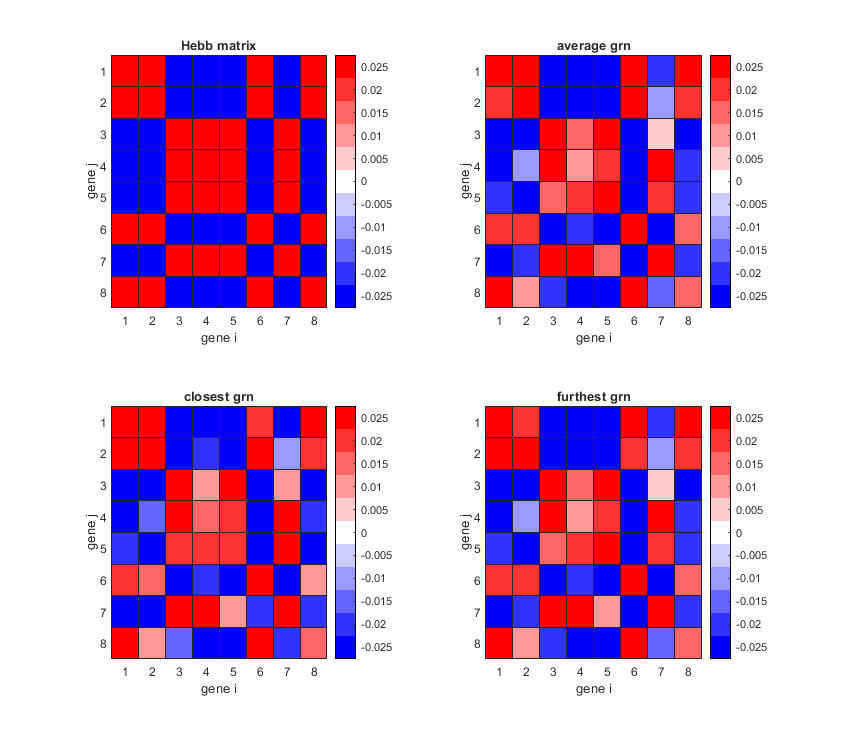
\includegraphics[width=\linewidth]{./img/results/pop100.png}
	\caption{Representation of gene regulation networks. Top left: Matrix calculated through Hebb's rule. Top right: Average gene regulation network, arithmetic mean of all gene regulation networks. Bottom left: Closest gene regulation network, most similar to Hebb matrix. Bottom right: Furthest gene regulation network, least similar to Hebb matrix.}
	\label{fig:pop100}
\end{figure}


\begin{appendix}
  \bibliography{Bericht} 
  \bibliographystyle{ieeetr}
\end{appendix}

\end{document}
